\documentclass[]{spie}  %>>> use for US letter paper
%\documentclass[a4paper]{spie}  %>>> use this instead for A4 paper
%\documentclass[nocompress]{spie}  %>>> to avoid compression of citations

\renewcommand{\baselinestretch}{1.0} % Change to 1.65 for double spacing

\usepackage{amsmath,amsfonts,amssymb}
\usepackage{graphicx}
\usepackage[colorlinks=true, allcolors=blue]{hyperref}

\title{LSST Data Management Software Development Practices and Tools}

\author[a]{Tim~Jenness}
\author[a]{Frossie~Economou}
\author[b]{Krzysztof~Findeisen}
\author[c]{Fabio~Hernandez}
\author[a]{Josh~Hoblitt}
\author[d]{Kian-Tat~Lim}
\author[d]{Fritz~Mueller}
\author[a]{William~O'Mullane}
\author[b]{Russell~Owen}
\author[e]{Stephen~R~Pietrowicz}
\author[f]{Pim~Schellart}
\author[a]{Jonathan~Sick}
\author[a]{Adam~Thornton}

\affil[a]{LSST Project Office, 950 N.\ Cherry Avenue, Tucson, AZ 85719, USA}
\affil[b]{University of Washington, Dept. of Astronomy, Box 351580, Seattle, WA 98195, USA}
\affil[c]{Centre de Calcul de l'IN2P3, USR 6402 du CNRS/IN2P3, 43 Bd. du 11 Novembre 1918, 69622 Villeurbanne Cedex, France}
\affil[d]{SLAC National Accelerator Laboratory, 2575 Sand Hill Rd, Menlo Park, CA 94025, USA}
\affil[e]{NCSA, University of Illinois at Urbana-Champaign, 1205 W. Clark St. Urbana, IL 61801}
\affil[f]{Department of Astrophysical Sciences, Princeton University, Princeton, NJ 08544}


\authorinfo{Further author information: (Send correspondence to T.J.)\\T.J.: E-mail: tjenness@lsst.org,\\  W.O'M: E-mail: womullan@lsst.org}

% Option to view page numbers
\pagestyle{empty} % change to \pagestyle{plain} for page numbers
\setcounter{page}{1} % Set start page numbering at e.g. 301

\begin{document}
\maketitle

\begin{abstract}
The Large Synoptic Survey Telescope (LSST) is an 8.4m optical survey telescope being constructed on Cerro Pach\'on in Chile.
The data management system being developed must be able to process the nightly alert data, 20,000 expected transient alerts per minute, in near real time, and construct annual data releases at the petabyte scale.
The development team consists of more than 70 people working in six different sites across the US developing an integrated set of software to meet the LSST requirements.
In this paper we discuss our agile software development methodology and our API and developer decision making process.
We also discuss the software tools that we use for continuous integration and deployment.
\end{abstract}

% Include a list of keywords after the abstract
\keywords{}


\section{INTRODUCTION}

The data management system\cite{2015arXiv151207914J} for the Large Synoptic Survey Telescope\cite{2008arXiv0805.2366I} has been under development since at least 2004\cite{2004AAS...20510811A}.
During that time a number of technologies have been adopted and our development practices have evolved as we transitioned from the research and development phase to construction.
The Data Management (DM) team is distributed, with representation from Princeton University, the University of Washington, the National Center for Supercomputing Applications at Urbana-Champaign, IPAC in Pasadena, the LSST Project Office in Tucson, and the SLAC National Accelerator Laboratory near Stanford University; along with some external contributions from CC-IN2P3 in Lyon, France.
Given this, it is important that comunication channels are open and easy to use and that our tools evolve as community standards evolve.
Being agile enough to be able to migrate from one tool to another during the lifetime of a project is key when the software, processes, and people, change over what will be a 25 year period once the 10-year survey completes.
For example, over the years we have migrated the codebase from Subversion to git; we have switched instant messaging from HipChat to Slack; we have migrated continuous integration from builbot on our own hosts to Jenkins running in the cloud; and we have moved documentation standards from Doxygen to Sphinx.

In the following sections we describe the current development practices for LSST DM.

\section{Agile Development}\label{sec:jira_ticket}

LSST data management follows a form of cyclic development often referred to as {\emph Agile} methodology. It is also beholden to organizations such as NSF which require a more traditional approach to project development such as the Earned Value Management System (EVMS).
We have presented this from both  the ESA and LSST perspective in SPIE previously  \cite{2014SPIE.9150E..1EG}.
In 2016  we presented a more complete approach for LSST to the problem of Agile in the earned value world \cite{2016SPIE.9911E..0NK}, here we provide just a brief update on that paper concentrating more on the Agile aspects.


\subsection{Management}
\cite{DMTN-020} provides a guide to the mechanisms underpinning LSST Data Management’s approach to project management, the reader is referred to to this for gory details as required.
Each institution in the DM team is still typically
responsible for 1 or more Level 2 WBS elements, and each institution has a Technical/Control Account Manager
(T/CAM) responsible for planning, estimating, monitoring and EVM reporting for that Level 2 WBS element.
The detailed management plan is in \cite{LDM-294}.

\subsection{Basic Assumptions}
The Project assumes that a full-time individual works for a total of
1,800 hours per year: this figure is \emph{after} all vacations, sick
leave, etc are taken into account. Staff appointed to ``developer''
positions are expected to devote this effort directly to LSST.

Appointment as a ``scientist'' includes a 20\% personal research time
allowance. That is, scientists are expected to devote 1,440 hours per
year to LSST, and the remainder of their time to personal research.

Our base assumption is that 30\% of an individual's LSST time (i.e. 540 hours/year for a developer, 432 hours/year for a scientist) are devoted to overhead for regular meetings\footnote{``Meetings'' include, for example, scheduled weekly team meetings, stand-ups, etc; major conferences or project meetings involving preparation, travel time, etc should be scheduled in advance and allocated Story Points}, ad-hoc discussions and other interruptions.
This is similar to the standard {\emph Agile} discount, however in the earned value world that must be accounted for and it is considered Level of Effort (LOE)


\section{Long Term Planning}
\label{sec:long-term-plan}

The plan for the duration of construction is embodied in:

\begin{enumerate}
\item
  A series of \emph{planning packages}, which describe major pieces of
  technical work. Planning packages are associated with concrete, albeit
  high-level, deliverables (in the shape of milestones), and have
  specific resource loads (staff assignments), start dates, and
  durations. The entire DM system is covered by around 100 of these
  planning packages.
\item
  \emph{Milestones} represent the delivery or availability of specific
  functionality. Each planning package culminates in a milestone, and
  may contain other milestones describing intermediate results.
\end{enumerate}

Planning packages are defined at the fourth level of the Work Breakdown Structure (WBS).

All WBS elements are related to the set of Data Management Products embodied in \citep{LDM-148} a high level summary of which is given in
Figure \ref{fig:prods}. Each product has a product owner to guide the agile development, this is frequently one of the Data Management Scientists.

\begin{figure}[htbp]
        \begin{center}
                 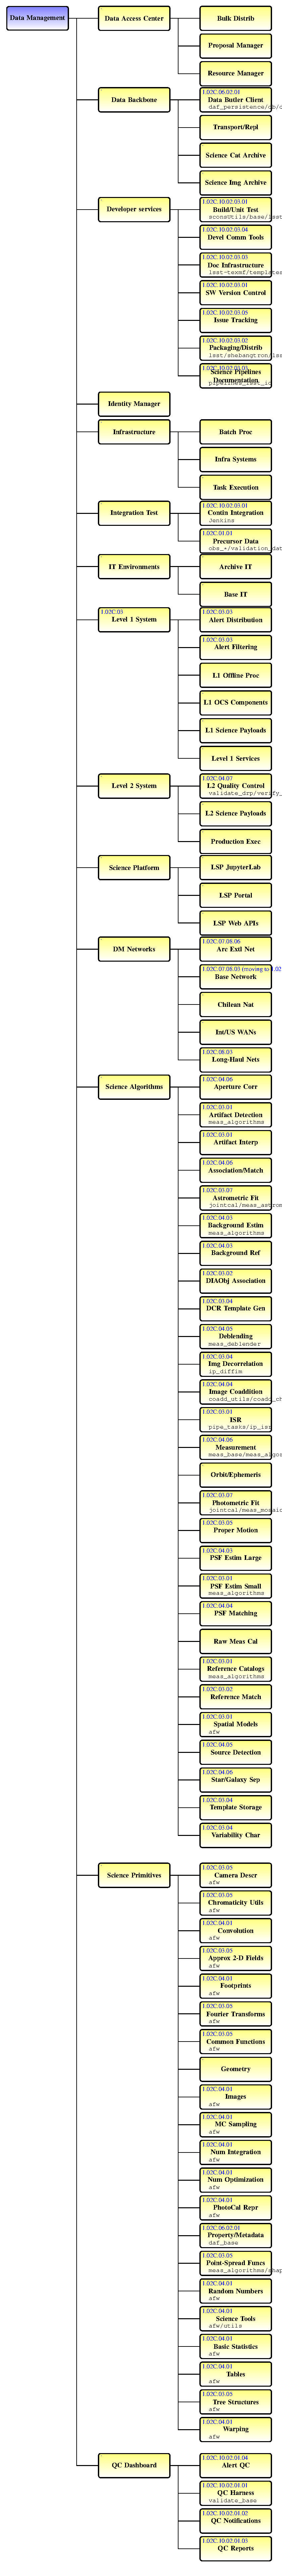
\includegraphics[height=19cm]{ProductTree}
                 \caption{DM product tree. \label{fig:prods}- there are over 200 products, this tree is to convey and idea of the products and is truncated to make it somewhat legible.
         }

         \end{center}
 \end{figure}

During the cycle planning process  effort is drawn from the budget embodied in the planning packages to generate the cycle plan, described in terms of epics in Jira.
Each epic itself has a particular budget.
This budget is subtracted from that available in the planning package at the point when the epic is defined.
Team members then add specific stories to these epics.

The Jira system is synchronized with the Primavera project management tool every three months using in house tools.

In order for the DM system to reach its science goals, new algorithmic or engineering approaches must sometimes be researched.
It is appropriate to budget time for this research work in planning packages.
Areas where successful delivery of the DM system is dependent on speculative research are a source of risk: where possible, the plan  also provides for a fallback option to be taken when research objectives are not achieved.
This may also lead to an entry in the risk register.



\section{Reporting }
Though the EVMS system is reasonable good for reporting it does not report well on Agile progress. Since  \citep{2016SPIE.9911E..0NK} we have undertaken a set of test driven milestones to show progress in Data Management.

Epics, stories, P6, milestones, EVMS.
How do we use product owners?
Test specifications and requirements.

How has this evolved since Kantor et al SPIE 2016? (kind of important that we link this SPIE paper to previous SPIE paper on Agile process).


\section{Model Based Systems Engineering}

LSST uses Model-Based System Engineering, with designs, requirements, and behavior described using the SysML language and stored within a database-backed tool, initially Enterprise Architect and now MagicDraw.
MagicDraw permits communication between teams through a unified model of the system.
It also allows for relatively easy maintenance of the requirements at all levels of the system as well as traceability between requirements and the system components that satisfy them.

Within the SysML language, there are specialized diagram types.
The Requirement Diagram documents requirements and their relationships.
Block Definition Diagrams highlighting interfaces and Internal Block Diagrams highlighting component breakdowns explicate the design of the system.
Activity Diagrams, Sequence Diagrams, State Machine Diagrams, and Use Case Diagrams show the system's intended behavior.
The MagicDraw tool allows these behavioral diagrams to be executed in a simulation mode to verify that the behavior is complete and correct.
All of this information is useful for the verification process.
Test cases are developed from requirements and behavior.

\subsection{Requirements}

Requirements are written using a combination of a formal specification, which uses verbs such as "shall" and "will" in a stylized manner, along with a description that explains the context and interpretation of the requirement.
Constraints are added to the requirement that document values of parameters used within the specification, along with their descriptions and units.
Each requirement is given a unique identifier generated based on its containing document and a monotonically-increasing sequence number.
This requirement id allows requirements to be safely referred to and linked together even if the containing document is reorganized or if a requirement is deleted or replaced by another.
Requirements document organization into sections is handled by grouping requirements into SysML packages.
Numbers prefixed to the titles of the packages and the requirements within them allow them to be sorted into a human-meaningful order.
These numbers are sequential within a containing package, not hierarchical, making renumbering and reorganization easier.
Requirements documents are generated using one of two custom macros, one for Microsoft Word documents and another for LaTeX documents.
The document generation macros strip off the sequential prefix numbers, allowing the word processing tools to create the hierarchical section and requirement title numbers.

\subsection{Requirements Documents}

Five levels of requirements documents are applicable to Data Management.
At the highest level, the LSST Science Requirements Document (SRD) sets out the overall scientific goals of the project in prose.
The LSST System Requirements are the project's formal response to the SRD, setting minimum, design, and "stretch" goals for requirement parameters.
The Observatory System Specification documents requirements and budgets based on a high-level design, in particular partitioning the LSST system into Telescope \& Site, Camera, Data Management, and Education \& Public Outreach subsystems.
At this level, the Data Products Definition Document provides a full specification of the data products to be delivered by the LSST system.
The Data Management System Requirements (DMSR) are the flowdown to DM specifically.
At the same level as the DMSR, Interface Control Documents (ICDs) specify the relationships between the different subsystems.
Finally, within the DM system, component requirements documents are used where appropriate to constrain designs and provide for internal verification.

\subsection{Flowdown}

One of the excellent features of MagicDraw is the ability to rapidly document the flowdown of requirements.
Using a table with higher-level requirements on one side and lower-level requirements on the other, the "refines" relationship between the latter and the former can be created by merely toggling an arrow within appropriate table cells.
Unfortunately, it is more difficult to use the SysML "copy" relationship in cases where the lower-level requirement happens to be identical to the higher-level one.
It has been necessary to manually copy the requirement text (and generate a new requirement id, of course).

Since system components are also present in the MagicDraw model, the tool also helps with recording which requirements apply to each component, and, conversely, which components are needed to satisfy each requirement.

\subsection{Conclusion}

Ultimately, SysML and MagicDraw have been most useful for systems engineering purposes at the LSST system level, rather than within the Data Management system itself.
While the tool is fully capable of recording component designs in diagrammatic language, adoption has been somewhat difficult; developers tend to prefer to work directly on code.
In its place, more limited diagrams are produced using other tools such as OmniGraffle, Gliffy (particularly with the Confluence plugin), LaTeX, Archi, and websequencediagrams.com.

\section{Software Development}

\subsection{Development Model}


The main focus of DM development is on the science pipelines packages\cite{2018PASJ...70S...5B} and the related support infrastructure, and the data access services and Qserv\cite{2011Wang:2011:QDS:2063348.2063364}.
The standardized EUPS-based build system currently knows how to build more than 230 packages, which includes packages supported by the simulations team\cite{2014SPIE.9150E..14C} and packages of external dependencies, and each of those packages has its own git repository on GitHub\footnote{\url{https://github.com/lsst}}.

For each of those DM git repositories we use a standard development methodology where the \texttt{master} branch is always releasable, in the sense that all unit tests pass and basic integration tests pass.
All work is done on feature branches that have the name \texttt{tickets/DM-nnnn} where \texttt{DM-nnnn} matches the corresponding Jira story or bug associated with the work.

Lots of small repositories.

Feature branches associated with Jira tickets.

Branch protection.

Rebase before merging.

\subsubsection{Comparison with other workflows}

git flow.


\subsection{Code Quality}

LSST DM is responsible for a large amount of code.

Qserv: 70,000 + 23000 comments C++ / 8k lines python: ~100k lines
Dax: 4000 lines python

% starlink_ast is exempted. Calculation was done on cleaned directories
% on 2018-04-02.
% perl ~/Downloads/cloc-1.72.pl $(cat manifest.txt  | awk '{print $1}')

lsst\_distrib consists of 120 packages/repos

--------------------------------------------------------------------------------
Language                      files          blank        comment           code
--------------------------------------------------------------------------------
Python                         1771          54192          95609         192982
C++                             859          21507          29472         108609
C/C++ Header                    555          14937          46781          42296




python: 288k
C++: 227k

Unit tests using pytest.

Flake8 clean with minor exceptions.\label{sec:flake8}

Code coverage.

Clang-format.

\subsection{EUPS}

Philosophy of eups

Implementation overview.

How we use EUPS.

Eupspkg.

\subsection{Building the software}

Use pip and pypi for infrastructure support packages.

How do we build science pipelines software in particular?

lsstsw and eups distrib.


\section{Communication}

\subsection{Slack}

The data management group uses instant messaging tools to answer questions, 
share code snippets and errors, and coordinate activities in real-time.  
Before using instant messaging, we would communicate primarily via e-mail or 
over the phone. While these tools do still have their place, being able to have 
conversations in a team-wide application has been very helpful. Discussions
happen with more team members participating, instead of just who happened to
be on a phone call or an e-mail thread. Questions and concerns have been able
to be answered much more quickly.  Site channels help coordinate discussions
useful to local teams.  We even have non-work related channels were we can
discuss various topics, which has sparked conversations about previously
unrealized common interests. It has been beneficial to team building and 
helped foster friendships.

We have used two different instant messaging tools in the last four years. The
first tool we used was HipChat. Besides the essential features expected
from an instant messaging client (such as discussion channels and one
to one direct messaging), we were also able to receive Jenkins and JIRA issue
notifications, which we found very helpful.

We used HipChat for two years and eventually started looking at other options 
because we found the user experience was, at times, inconsistent and 
frustrating. One of the most significant issues was how it managed unread
messages. If the user left the application, HipChat did not maintain where the
user was in the message chain. When the tool restarted, it required the user
to scroll back through messages to pick up where they left off. Notifications
were erratic, and sometimes would arrive late or not at all. Some users
particularly liked features such as video chat, while other users found this
feature unstable and resorted to using other video chat services such as Google 
Hangouts. 

After a brief testing period, we decided to transition to Slack, which we
continue to use today. The move from HipChat to Slack was straightforward,
although we did lose the discussion history from HipChat.  At first, we 
thought this would be an issue, but in practice, we rarely search history older
than a couple of weeks.  We have had difficulties in balancing when to 
archive these discussions for the community.  We've also had some problems
making sure that decisions made within a Slack conversation were
distributed to more team members, since everyone may not have been in the 
channel at that time.  We continue to improve our efforts in this regard by 
starting RFC's or Confluence discussions to distribute information more widely.

Slack initially didn't have video chat when we switched from HipChat, but
it does now.  We use this for ad-hoc calls for the channel, which has been
easier than coordinating a call via Google Hangouts or BlueJeans.

When we made the switch, we wanted to take the opportunity to normalize the
users' chat names to match the names used on GitHub, which would have 
simplified how we notified users of software build failures.  It proved
difficult to coordinate, so we let our Jenkins bot do the translation between
their GitHub ID and their Slack account.

Slack offers of HipChat's functionality and improves several features. Slack 
has several options on how unread messages are handled and displayed, allowing
users to choose how the application behaves when the application restarts. 
Users can decide how to handle unread messages either showing them where the
application was last used, or by marking them already read.

Other features include direct messaging can be set up for small groups,
instead of creating a public chat room for an ephemeral discussion topic.
We create temporary channels for members to communicate during workshops and 
conferences, which helps team members coordinate while on-site and to involve
people who aren't attending.  This paper itself was even organized
within a Slack channel, allowing us to discuss it and to get automatic
notifications of changes to it via the GitHub Slack bot.

Previews of URLs, global and per channel notification preferences and an 
API to integrate third-party or custom chat-bot apps. One of those apps, 
sqrbot, is discussed in the next section.  

Other subsystems within LSST which either had already been using HipChat or
were beginning to explore instant messaging services have also transitioned to 
Slack. We expect this to be of great benefit to us as we integrate the work 
from the LSST sub-systems.

\subsubsection{Chat Ops}

DM-SQuaRE is using a Slack chatbot called ``sqrbot'' to make some tasks
easier. Currently it performs a range of functions, from returning the
status of various infrastructure machines to creating technotes to
monitoring whether metrics in our processing stack have changed between
CI builds; it also listens for mentions of Jira tickets, and when it
hears one, posts a link to that ticket.

All of these tasks are frequently requested actions that formerly
required breaking workflow.  Either (as with technote creation) the
requestor would have to interrupt someone else in order to get the work
performed, or they'd have to interrupt their own workflow to, for
instance, copy the ticket name, go to Jira, and search for the ticket.
With sqrbot, the requestor can simply ask sqrbot in a Slack channel for
the information (or creation of a technote skeleton, etc.) and get
immediate gratification without needing to task-switch or interrupt
a co-worker.

The basic architecture is simple: sqrbot is simply a collection of hubot
scripts running as a Slack bot, which in turn drive microservices,
written in Python and implemented using the Flask framework.  These
microservices have an API that responds with JSON, so the job of sqrbot
is simply to accept commands, create appropriate HTTP transactions, and
then reformat the output into a conversational format.  The whole
assembly runs in a Kubernetes cluster.


\subsection{Community forum}

Description of purpose and usage.

\subsection{Confluence}

Transient information. Not used to document processes or for reports.

* Planning hack sessions?

* Integrating Jira tickets into confluence pages to indicate progress.

Meeting minutes

* Short term actions -- migrate to Jira if long term.


\section{Documentation}

\subsection{Types of Documentation}

Data Management creates a variety of documentation for audiences, and with different purposes.
Broadly, we break documentation efforts into two categories: project documentation, and user documentation.
Project documentation is a tree of requirements documents, interface control documents, design documents, and test reports that aides the construction project.
User documentation, on the other hand, is a deliverable that we ship alongside our software and services to either the scientific community or future developers and operators.

\subsubsection{Project documentation}

\paragraph{Documentation tree}

DM creates project documentation that fits within LSST's overall Document Management Plan (LPM-51).
As is standard practice, we organize the collection of project documents in a tree.
LSST Project Management and Systems Engineering requirements documents form the tree's trunk, along with interface control documents that DM collaborates on with other LSST subsystems.
These flow into Data Management requirements documents for each DM product: Database (LDM-555), Middleware (LDM-556), Science Platform (LDM-554), and Data Management System Design (LDM-148).
From these, we maintain design documents: Database Design (LDM-135), Middleware Design (LDM-152), Science Platform Design (LDM-542), Services and Infrastructure Design (LDM-129), Pipeline Design (LDM-151), and Network Design (LSE-78).
Then from each design document, we maintain test specification documents.
Overall, the DM Validation and Test Plan (LDM-503) coordinates these test specifications. Finally, we write test reports that implement the test plans.

We have processes managing project documents and revisions.
The DM Change Control Board (DM-CCB) reviews documents and revisions before they become the accepted baseline.
The DM-CCB also reviews test reports and approves those that specifically refer to formal milestones in the LDM-503 verification and test plan.

\paragraph{Technical notes}

We recognized that DM team members needed to write documents as a means of communication within the project.
These documents might be design proposals, summaries of data processing experiments, or descriptions of a new internal tool or service.
This content does not fit within the formal document tree, nor does it require oversight from the DM CCB.
Technical notes fit this niche for DM.

Since the defining characteristic of technical notes is the editorial independence of their authors, we sought to automate as much of the maintenance surrounding these documents as possible.
By allowing an author to create a new document and publishing it without either seeking permission or waiting on a human coordinator, we maximize the likelihood that DM team members will choose to share information through technical notes.
Thus we have implemented a self-service system based on ChatOps that allows any Data Management staff member to create and publish a technical note (++add cross-reference++).
These technical notes are edited on github.com and published as websites, and in the future, we plan to make these documents readily citable with DOIs and listings in archives.

As a cultural benefit, we see technotes as a way for junior members to gain exposure within the project, and beyond, by publishing a bylined article featuring their contributions.

\paragraph{Developer Guide}

The DM team is large and distributed, yet we need to work coherently.
An effective way to promote this is through strong documentation of internal processes and policies.
These range from a description of how we communicate, to the development workflow, code style guides, and user guides for internal services.
While we could conceivably publish this information as a kind of project documentation (see above), the content of the Developer Guide doesn't fit into a narrative format.
Instead, the content is made up of isolated, yet inter-linked, how-to pages and guides.
Thus we chose to publish our Developer Guide as a website (https://developer.lsst.io), using the same systems as we do for our user documentation.
DM team members are encouraged to contribute improvements to the developer guide through GitHub.
We use GitHub pull requests to get feedback on contributions and provide approval for changes to controlled pages such as coding style guides.

\subsubsection{User documentation}

User documentation describes what is built, and most importantly, how to operate it.
Thus we consider user documentation to be a deliverable product of the LSST construction project, on par with the software itself.

At the time of this publication, most DM effort towards user documentation have gone into the LSST Science Pipelines product (https://pipelines.lsst.io) and user guides for internal tooling.
The LSST Science Platform is the second major documentation project.
DM will also lay the groundwork for documentation of both the data releases and prompt products.

We begin a new user documentation project by studying the nature of the product user needs.
Then we work towards an information architecture plan that maps out topics in the user documentation project.
As described by Baker (CITE), topics are self-contained (though highly interlinked) articles that conform to a type.
The general categories of topic types are concept guides, tutorials, how-to guides, and references (cite).
This exercise not only allows us to systematically map the content needed to document a project but also understand the infrastructure needed to support each topic type (such as the tools needed to generate an API reference, or the tools needed to deliver and test a tutorial).
The DMTN-030 technical note is our living design for the LSST Science Pipelines user documentation.

\subsection{How we build documentation}

* LSST the Docs (versioned, web-based, continuous delivery)

* LaTeX documentation system

* Sphinx-based user documentation

-- breathe/numpydoc/doxygen


\section{Decision Making Process}

\subsection{RFCs}

\subsection{Change Control Board}

\section{Continuous Integration}

Jenkins.\label{sec:jenkins}

Travis for simpler items (yaml file validation, flake8 tests)

\section{Continuous Deployment}

\subsection{Deploying Science Pipelines Releases}

Weekly and daily releases. \label{sec:releases_weekly}\label{sec:releases_daily} Publish to eups server and docker container.

\subsection{Case Study: Deploying Qserv}

Docker etc.

Distributed service application; multiple flavors of containers for various parts of the service are built by
CI.
TravisCI uses containers to run multi-node integration test suite on each branch commit and PR.
Container deployment to bare-metal clusters is currently done with ad-hoc scripting, but we are moving to k8s.
Discussion of some development and testing leverage we are looking to get from k8s.

\subsection{Case Study: Deploying releases to JupyterLab}

Link to main JupyterLab paper by Frossie et al.

\subsection{Deployment at IN2P3}

As part of its preparation for contributing to the annual LSST data release processing during the operations phase, since 2015 IN2P3 computing center (CC-IN2P3) has been consistently deploying releases of the LSST software stack as soon as they are available.

Two mechanisms have been used for this continuous deployment. First, a deployment of both stable and weekly releases of the LSST software is made on a networked file system, accessible from all the hosts in both the login and batch farms of the site. The second mechanism used is CERN's CernVM File System (CernVM-FS) (TODO: cite). CernVM-FS is a HTTP-based mechanism for distributing software packages over a wide area network. It is implemented as a POSIX read-only file system in user space with intelligent cache management: this file system can be mounted on a scientist's personal computer as well as on a compute node of a batch farm. This mechanism is well suited to guarantee that exactly the same software is used by scientists during the development of their own software on top of LSST's and the one used when executing their software at scale on CC-IN2P3's data processing platform.

We adopted a deployment policy which has proven effective over the period we have been performing this process. Each deployment, be it of a weekly or a stable release, is as self-contained as possible. In other words, each release includes most of its software dependencies, including the Python interpreter each release is built for. In addition, a select set of third party packages is deployed to extend the LSST software, making sure that no dependencies of the LSST stack are modified. The C++ compiler and runtime library, which the LSST software depends on, are not included in each release but are pre-installed in all hosts of the site.

Each extended release is installed from binaries (if available) or from sources (TODO: reference section 9.1). It is typically composed of about 150.000 files and directories which aggregated take about 13GB of  storage. At least the 12 most recent weekly releases and all stable releases are available at any given moment. Removing an obsolete release is straightforward: recursively removing the directory where the release is installed removes it and all its dependencies, without affecting other installed releases.

IN2P3 scientists, the end users of this continuous deployment, use the installed releases in several ways. They prepare batch jobs which use the LSST software stack for processing simulated or precursor data. They also use those releases to launch Python notebooks for data exploration, visualisation and rapid prototyping: they can easily choose the version they want to use for a particular notebook and launch it for execution on any host of the CC-IN2P3 login farm, which are co-located with the datasets they want to process. stackyter\footnote{\url{http://stackyter.readthedocs.io}}, a convenience SSH wrapper is typically used for seamlessly and securely launching notebooks at CC-IN2P3 using the end user's credentials.

Dependable access to a data processing facility where scientists can use recent LSST software to process co-located datasets of significant size, without worrying with the technicalities of software deployment, has been proven very effective. It allows them to test new capabilities of the software and promptly detect regressions and provide feedback to the developers. The policy of removal of older weekly releases encourages them to continuously validate their own software against very recent LSST software.

TODO: make sure this section is consistent with section 9.1.

%%% NOTE: to reference other section use \autoref{sec:eups}


\section{Conclusion}

Distributed team. Finding balance. Blah blah.


\acknowledgments % equivalent to \section*{ACKNOWLEDGMENTS}

This material is based upon work supported in part by the National Science Foundation through Cooperative Agreement 1258333 managed by the Association of Universities for Research in Astronomy (AURA), and the Department of Energy under Contract No.\ DE-AC02-76SF00515 with the SLAC National Accelerator Laboratory.
Additional LSST funding comes from private donations, grants to universities, and in-kind support from LSSTC Institutional Members.

% References
\bibliography{spie-10707-10} % bibliography data
\bibliographystyle{spiebib} % makes bibtex use spiebib.bst

\end{document}
